\subsection{Umfrage}\label{sec:survey}
Die in \autoref{sec:interview} aufgestellten Hypothesen werden in diesem Kapitel näher untersucht. Die empirische Methode der Online-Umfrage\cite{value-online-survey} ermöglicht es, die im Interview ermittelten Daten zu quantifizieren. Die Aussagekraft einer Online-Umfrage ist vergleichbar mit Papier-Bleistift-Befragungen\cite{online-marktforschung}. Mithilfe der quantitativen Daten können, anhand von Methoden der statistischen Analyse, neue Erkenntnisse erschlossen werden.
Die Stichprobe wird innerhalb mehrerer Discord\footnote{Ein soziales Medium, welches Personengruppen in Server unterteilt\cite{discord}}-Server durchgeführt. Jede Person auf dem Discord-Server besitzt die gleiche Wahrscheinlichkeit an der Online-Umfrage teilzunehmen und somit Teil der Stichprobe zu sein. Das Auswahlverfahren erfolgt also zufällig. Diese Server richten sich primär an Personen, welche ein Interesse an Digimon-Videospiel Remakes\footnote{Ein Remake beschreibt in diesem Kontext die Anpassung eines Videospiels zum Zweck der Modernisierung.} oder Digimon im Allgemeinen aufweisen. Aus diesem Grund kann die Wahrscheinlichkeit, dass eine Person Kontakt mit Digimon World hat, höher sein. Die Umsetzung der Online-Umfrage versichert auch, dass die erhobenen Daten anonymisiert sind.\\

Der Aufbau des Fragebogens gliedert sich in drei Teile. Der erste Teil der Umfrage erhebt demografische Daten und lockert mit einfachen Eingangsfragen die Umfrage auf. Dies erfolgt analog zu den ersten beiden Phasen des Interviewleitfadens aus \autoref{table:interview-guideline}. Der zweite Abschnitt ermittelt allgemeine Informationen zum Spiel. Diese Informationen geben in der statistischen Analyse Aufschluss darüber, inwiefern unterschiedliche Nutzergruppen die einzelnen Hypothesen bewerten. Ebenfalls beinhaltet die Umfrage zwei Freitext-Felder, um weitere qualitative Daten bezüglich des Kampfsystems zu erfassen. Dieses Feedback wird in der späteren Implentierungsphase berücksichtigt. Abschließend bewerten die Teilnehmenden im letzten Teil der Umfrage die festgestellten Hypothesen. Diese Bewertung erfolgt anhand einer linearen Skala von eins bis fünf, wobei eins für volle Ablehnung und fünf für volle Zustimmung steht.  \\

Intervalle zwischen den einzelnen Antwortmöglichkeiten sind nicht als gleich zu interpretieren. Allerdings ist es möglich, diese Antwortmöglichkeiten in eine sinnvolle Reihenfolge zu bringen. Aus diesem Grund ist von einer Ordinalskala auszugehen\cite[S.11]{elementare-stochastik}. Dies bedeutet, dass nur die logischen Operationen einer Nominalskala ($=$/$\neq$) und Vergleichsoperatoren ($<$/$>$) anwendbar sind. Die messbaren Eigenschaften belaufen sich auf Untersuchung der Häufigkeit oder Rangfolge.\\

Die Online-Umfrage wird mithilfe von Google Formulare\cite{google-forms} durchgeführt und die dabei enstehenden Datensätze werden anschließend als \ac{CSV} exportiert. Die \ac{CSV} beinhaltet 80 Antworten, wobei 79 Personen das Spiel gespielt haben und eine Person das Spiel nicht gespielt hat. Diese Person wird aus der Ergebnismenge entfernt. Ebenfalls werden die qualitativen Daten bezüglich des Kampfsystems aus der \ac{CSV} entfernt. Die relevanten Daten werden mithilfe der Programmiersprache R\cite{r-project} analysiert und die Ergebnisse dieser Analyse werden im Folgenden vorgestellt. \\

\begin{figure}[H]
\centering
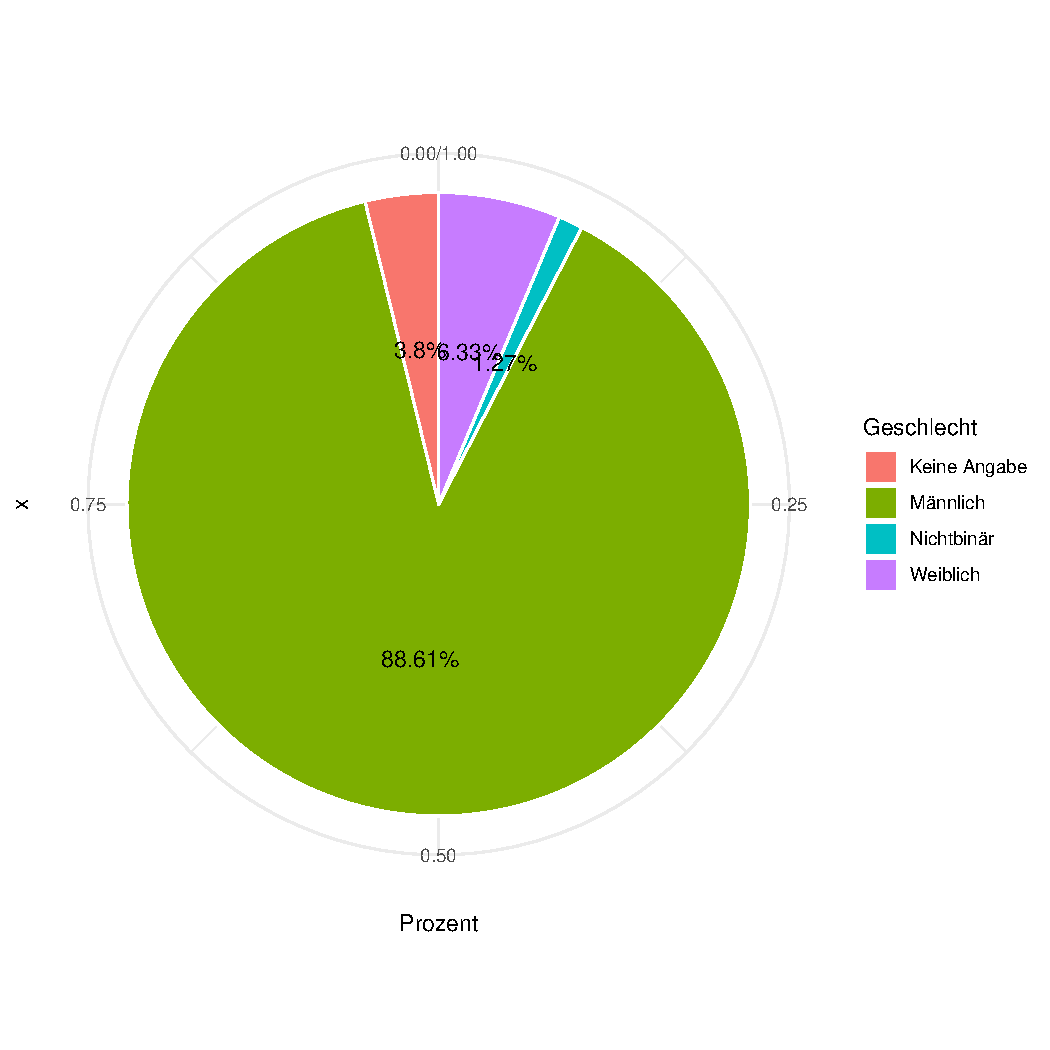
\includegraphics[width=0.7\columnwidth]{figures/plots/gender.pdf}
\caption{\label{fig:piechart-gender} Geschlecht der befragten Personen}
\end{figure}

Das Kreisdiagramm in \autoref{fig:piechart-gender} zeigt, dass sich 88,61\% der befragten Personen mit dem männlichen Geschlecht identifizieren. An dieser Stelle sei angemerkt, dass das Ergebnis der Auswertung mehrere Ursachen haben und die Ergebnisse bei Befragung einer anderen Personengruppe anders ausfallen kann. Die ausgewählten Discord-Server enthalten überwiegend männliche Mitglieder, weswegen die Stichprobe voreingenommen sein kann. Ebenso kann die Zielgruppe von Digimon oder Digimon World 1 bewusst primär das männliche Geschlecht sein. Dies wird von der Aussage der interviewten weiblichen Person gestützt, dass diese sich nicht zugehörig zur Zielgruppe fühlt[P2, 658-660].\\

\begin{figure}[H]
\centering
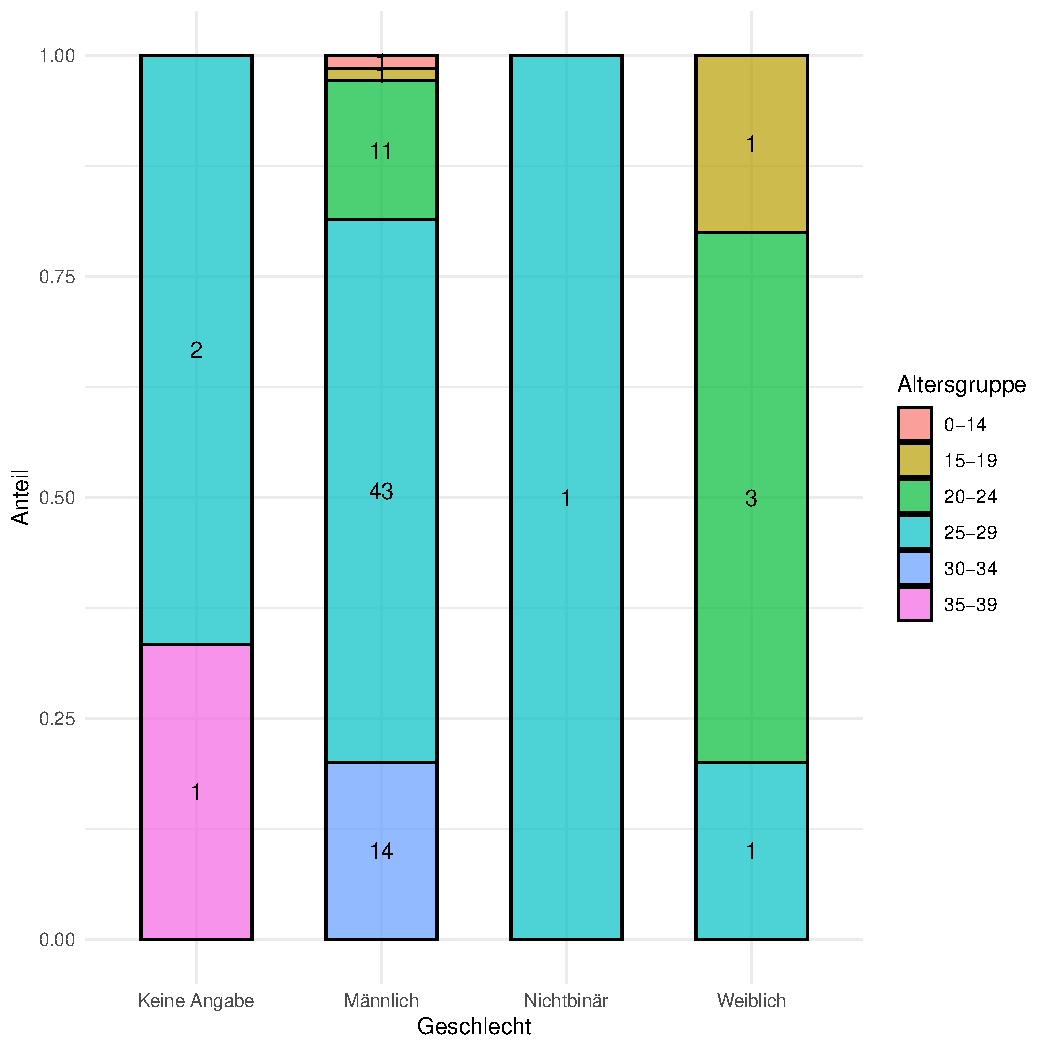
\includegraphics[width=0.65\columnwidth]{figures/plots/age_gender.pdf}
\caption{\label{fig:age-gender} Altersgruppen innerhalb der Geschlechter}
\end{figure}

\autoref{fig:age-gender} zeigt die Verteilung der Altersgruppen innerhalb der Geschlechter. Das Modell verdeutlicht, dass die Altersgruppe der Personen von 25-29 Jahren überwiegt. Ebenfalls existieren keine befragten Personen in der Altersgruppe über 39 Jahren. Es ist fraglich ob dies mit der Zielgruppe von Discord oder der tatsächlichen Zielgruppe von Digimon World zusammenhängt. Lediglich eine einzige Person in der Altergruppe von 0-14 Jahren hat an der Umfrage teilgenommen. Dies ist widersprüchlich, wenn die Klassenbreite\footnote{Die Klassenbreite $\Delta$ bezeichnet die Differenz der oberen und unteren Klassengrenze\cite[S.27]{elementare-stochastik}} von 14 betrachtet wird, da diese eine größere Gruppe von Personen eingrenzt als die anderen Altersklassen. Allerdings kann die geringe Teilnahme dadurch erklärbar sein, dass die Discord-Nutzungsbedingungen nur Nutzer im Alter von mindestens 13 Jahren erlauben. Aufgrund dieser Tatsache kann die tatsächliche Klassenbreite nur zwei betragen. Bei den weiblichen Teilnehmern scheint die Altersgruppe im Vergleich zu den anderen Geschlechtern jünger zu sein. Allerdings ist die Anzahl der befragten weiblichen Personen zu gering und es kann nur spekuliert werden, weswegen dies der Fall ist. \\

Im Januar 1999 bis Juli 2001 wurde Digimon World in unterschiedlichen Regionen veröffentlicht. Innerhalb dieser Jahre wurde ebenfalls der Anime\footnote{In Japan produzierte Zeichentrickserie} Digimon Adventure in vielen Regionen veröffentlicht\cite{imdb-release}. Digimon Adventure richtet sich primär an Kinder\cite{mal-adventure} und wurde unter anderem mit dem Begriff Shounen getaggt\cite{anidb-adventure}. Der Begriff Shounen bezeichnet im japanischen die Zielgruppe von jungen männlichen Personen\cite{manga-brunner}. Die starke Verteilung innerhalb der Altersgruppe von 25-29 Jahren kann erklärt werden, wenn diese zeitlich zum Zeitpunkt des Releases von Digimon World verlagert wird. Wenn die Altersgruppe 25-29 um 20 Jahre zurückversetzt wird, beträgt die neu errechnete Altersgruppe 5-9 Jahre. Aufgrund der Tatsache, dass die Altersgruppe mit der Zielgruppe von vor 20 Jahren übereinstimmt, ist davon auszugehen, dass viele Teilnehmer deswegen in diese Altersgruppe fallen, weil diese das Spiel vor 20 Jahren bereits gespielt haben. Ebenfalls lässt sich der hohe männliche Anteil in der Verteilung durch diese Zielgruppe erklären. \\

\begin{figure}[H]
\centering
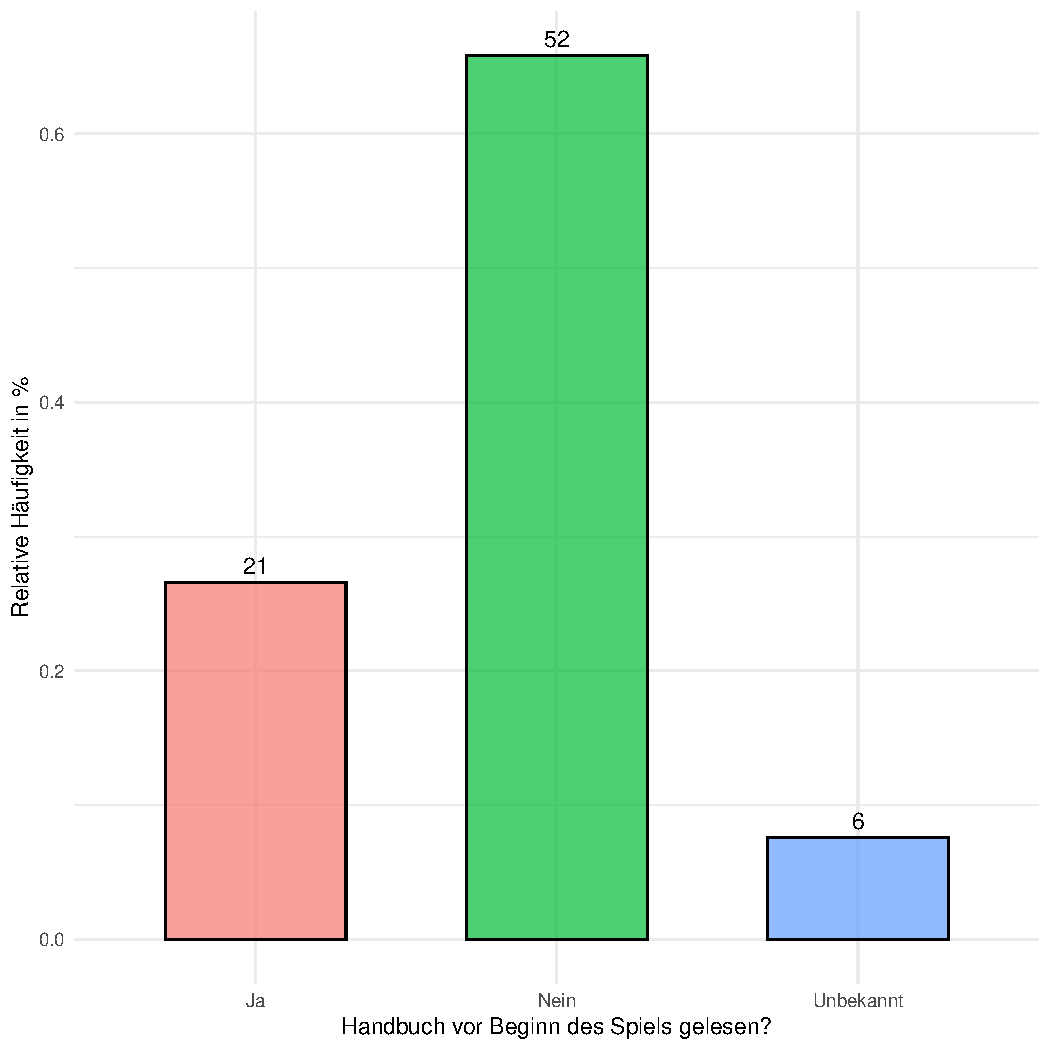
\includegraphics[width=0.65\columnwidth]{figures/plots/manual.pdf}
\caption{\label{fig:manual} Anzahl der Personen, welche das Handbuch gelesen haben}
\end{figure}

Im Versuchsaufbau vom Interview in \autoref{sec:interview} ist aufgefallen, dass zwei Drittel (66,66\%) der interviewten Personen sich das Handbuch nicht angesehen haben. Es wurde die Annahme gemacht, dass der Versuchsaufbau des Interviews irreführend sein könnte. Das Säulendiagramm in \autoref{fig:manual} zeigt allerdings deutlich, dass 52 der 79 befragten Personen (65,8\%) ebenfalls das Handbuch vor Beginn des Spiels nicht gelesen haben. Es spricht nichts dagegen, dass Personen im Verlauf des Spiels zum Handbuch greifen. Allerdings verfehlt dies den Sinn und kritische Informationen könnten erst zu einem späteren Zeitpunkt für die Spielenden verfügbar sein.\\

\definecolor{LightGray}{gray}{0.9}
\begin{listing}[H]
\caption{Analyse in R}
\label{lst:correlation}
\begin{minted}[
bgcolor=LightGray,
framesep=2mm,
baselinestretch=1.2,
fontsize=\footnotesize,
linenos,
]{r}
if (!require('pacman')) install.packages('pacman')
p_load(pacman, tidyverse, ggpubr, corrplot)

csv_df <- read.csv('data/results.csv')
df <- csv_df[, 14:30]

for (i in 1:17) {
  names(df)[i] <- sprintf('H%s', i)
}

correlations <- round(cor(df, method = 'spearman'), digits = 2)
corrplot(correlations, method = 'circle', type = 'upper')
correlations[abs(correlations) < 0.5 | correlations == 1] <- ''

for (i in 1:20) {
  df[, i] <- round(jitter(df[, i], factor = 0.3), digits = 3)
}

ggscatter(
  df,
  x = 'H11',
  y = 'H12',
  add = 'reg.line',
  conf.int = TRUE,
  cor.coef = TRUE,
  cor.method = 'spearman',
) +
  theme_minimal()
\end{minted}
\end{listing}

\autoref{lst:correlation} zeigt beispielhaft eine in der Arbeit ausgeführte Auswertung in R.
Zunächst werden benötigte Pakete mit dem Paketmanager pacman\cite{rdoc-pacman} geladen. Anschließend werden die Daten in Zeile vier bis neun, aus der zuvor exportierten \ac{CSV}, geladen, in der Variable \texttt{df}\footnote{Üblich abgekürzter Variablenname für \texttt{data\_frame}} gespeichert und korrekt umbenannt. Im Anschluss daran werden die Korrelationen zwischen den einzelnen Hypothesen nach Spearmans Korrelationskoeffizienten $\rho$ berechnet und auf zwei Nachkommastellen gerundet. Spearmans Korrelationskoeffizient wird verwendet, um den Zusammenhang zwischen zwei rangskalierten Variablen zu bestimmten\cite{statistik-datenanalyse}. Die berechnete Stärke des monotonen Zusammenhangs befindet sich im Intervall $[-1, 1]$, wobei $0$ kein Zusammenhang und $-1$ oder $1$ vollständiger monotoner Zusammenhang bedeutet. An dieser Stelle sei angemerkt, dass Korrelation nicht gleich Kausalität bedeutet\cite[S.64]{elementare-stochastik}. Es handelt sich zunächst lediglich um einen mathematischen Zusammenhang. Diese Werte sind als symmetrische 17x17 Matrix in der Variable \texttt{correlations} gespeichert. \\

\begin{figure}[H]
\centering
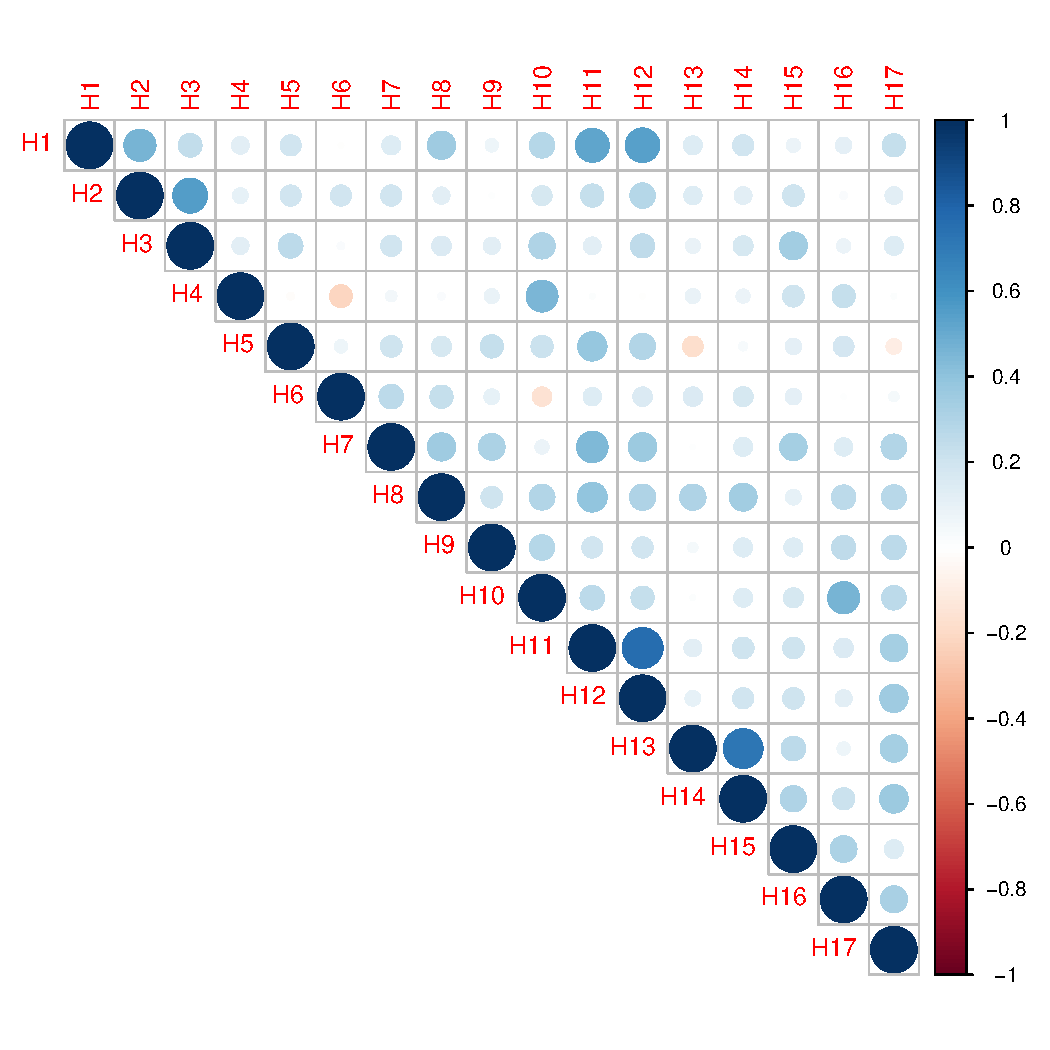
\includegraphics[width=0.65\columnwidth]{figures/plots/correlation.pdf}
\caption{\label{fig:correlations} Korrelationsmatrix nach Spearmans $\rho$}
\end{figure}

Anschließend stellt Zeile zwölf im \autoref{lst:correlation} die Korrelationsmatrix, wie in \autoref{fig:correlations}, grafisch dar. Aufgrund dessen, dass die Korrelationsmatrix symmetrisch ist, wird diese mithilfe der Option \texttt{type = upper} nur auf einer Seite der Hauptdiagonale erzeugt.
Das Ausblenden einer Seite dient der Übersicht. Entlang der Hauptdiagonalen ist der Zusammenhang zwischen einer Hypothese mit sich selbst immer 1. Jede Hypothese korreliert folglich perfekt mit sich selbst. Diese Information bringt allerdings keinen Mehrwert.\\

Zeile 13 aus \autoref{lst:correlation} löscht die Werte der Hauptdiagonalen und aller Elemente, dessen absoluter Wert unter 0.5 fällt. Diese Filterung wird durchgeführt, weil in dieser Arbeit nur die stärker korrelierenden Werte betrachtet werden\cite{cohen-power}. Nach Ausführen der Funktion beinhaltet die symmetrische Matrix \texttt{correlations} nur noch zehn anstelle von 289 Einträgen. Aufgrund der Symmetrie bedeutet dies, dass fünf Hypothesen einen Korrelationskoeffizienten von über 0.5 oder unter -0.5 betragen. \\

\begin{figure}[H]
\centering
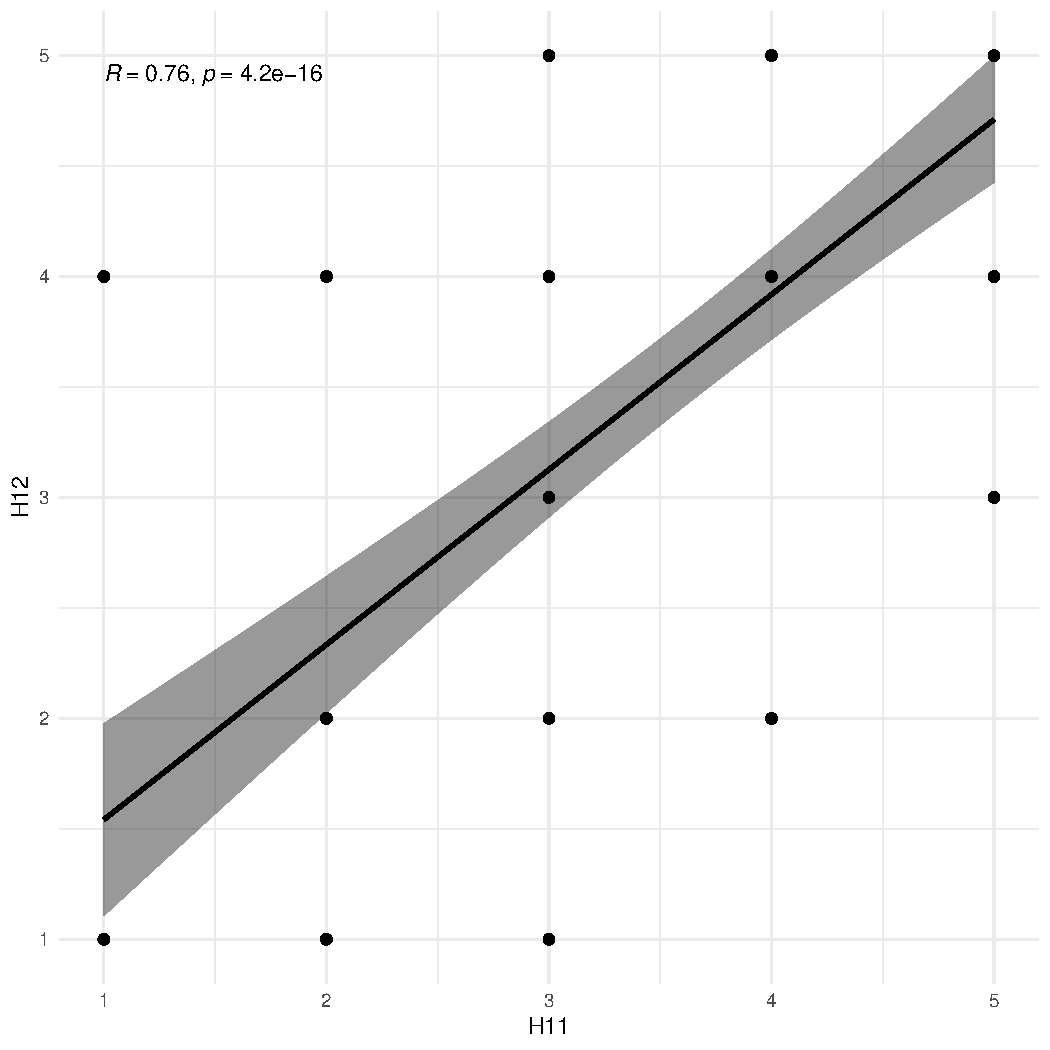
\includegraphics[width=0.65\columnwidth]{figures/plots/without_jitter.pdf}
\caption{\label{fig:without_jitter} Streudiagramm - Korrelation zwischen H11 und H12}
\end{figure}

Mithilfe der Funktion \texttt{ggscatter} kann das Streudiagramm aus \autoref{fig:without_jitter} erstellt werden. Diese Funktion wird in Zeile 19-28 in \autoref{lst:correlation} verwendet. Das Diagramm stellt die Abhängigkeit der Hypothesen H11 und H12 dar. Der errechnete Korrelationskoeffizient R nach Spearman beträgt 0,76. Der p-Wert in \autoref{fig:without_jitter} misst die Wahrscheinlichkeit, dass ein Unterschied zwischen zwei, in der Arbeit ermittelten, Hypothesen zufällig sein könnte. Wenn dieser Wert unter dem festgelegten Signifikanzniveau $\alpha$ von 0,05 liegt, ist das Ergebnis mit einer Fehlerwahrscheinlichkeit von p signifikant\cite[S.350]{elementare-stochastik}. Dies ist hier der Fall, weswegen davon auszugehen ist, dass die Korrelation zwischen H11 und H12 nicht zufällig ist. Die Fläche neben der Regressionsgeraden gibt die Wahrscheinlichkeit an, dass ein Wert mit 95\%-iger Wahrscheinlichkeit in diesen Bereich fällt.\\

Die Darstellung von \autoref{fig:without_jitter} ist allerdings irreführend, weil gleiche diskrete Werte sich überlagern und nicht unterschieden werden können. Aus diesem Grund werden die Werte aus \texttt{df} mit der Funktion \texttt{jitter}\cite{jitter} zufällig, um einen kleinen Faktor, verändert. Diese Funktion wird für alle Werte in \texttt{df} angewendet und befindet sich in Zeile 15-17 in \autoref{lst:correlation}. Dies hat zur Folge, dass sich der R- und p-Wert ebenfalls verändern und das Resultat verfälscht wird. Diese Herangehensweise wird hierbei nur verwendet, um die Daten anschaulicher darstellen zu können.

\begin{figure}[H]
\centering
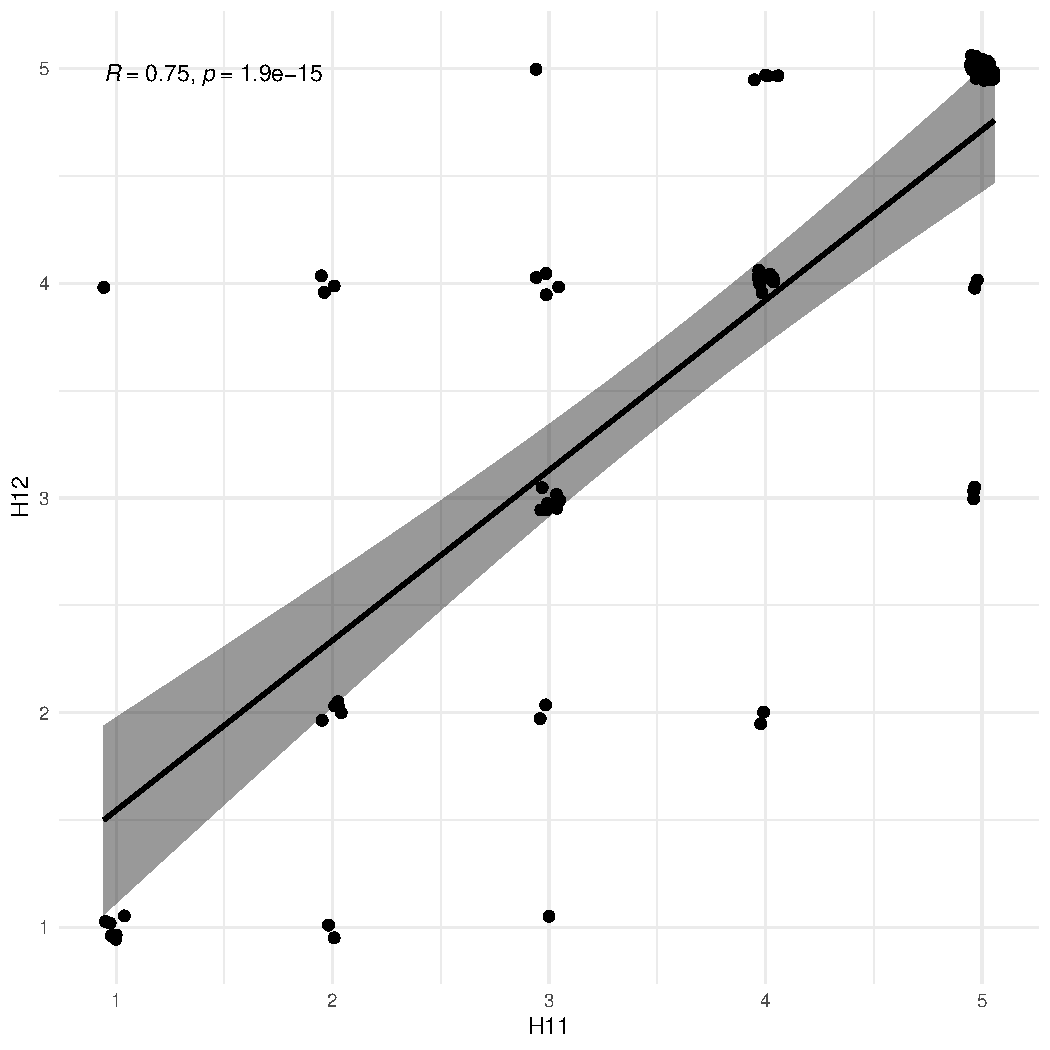
\includegraphics[width=0.65\columnwidth]{figures/plots/h11_h12.pdf}
\caption{\label{fig:h11_h12} Verwackeltes Streudiagramm - Korrelation zwischen H11 und H12}
\end{figure}

Der positive Effekt dieser Herangehensweise lässt sich in \autoref{fig:h11_h12} erkennen. Nach der Anwendung der Funktion \texttt{jitter} lassen sich gleiche Werte nun unterscheiden, weil diese sich nicht überlagern. Die neu entstandenen Punktewolken verdeutlichen die Häufigkeiten der Antworten. Alle weiteren, auf diese Art und Weise erzeugten, Graphen befinden sich im Anhang in \autoref{sec:scatterplots}. Dort befindet sich auch die \autoref{table:correlations-overview}, welche die errechneten Werte ohne Anwendung der Funktion \texttt{jitter} zeigt.\\

Vier der fünf ermittelten Korrelationen deuten darauf hin, dass Personen, welche an zusätzlichen Informationen im Spiel interessiert sind, sich diese Informationen auch an anderen Stellen im Spiel wünschen. Das bedeutet, dass davon auszugehen ist, dass eine Zielgruppe, welche sich allgemein mehr Informationen in Digimon World wünscht existiert. Das gleiche Prinzip gilt bei der Korrelation zwischen neuem Aussehen des Charakters und der Auswahl des Geschlechts (siehe H13-H14 in \autoref{table:correlations-overview}). Hier wird deutlich, dass Personen an der Personalisierung des Charakters im Allgemeinen interessiert sind. Aus diesem Grund wird im Entwicklungsprozess darauf geachtet, dass korrelierende Funktionen gut aufeinander abgestimmt sind.\\

\begin{figure}[H]
\centering
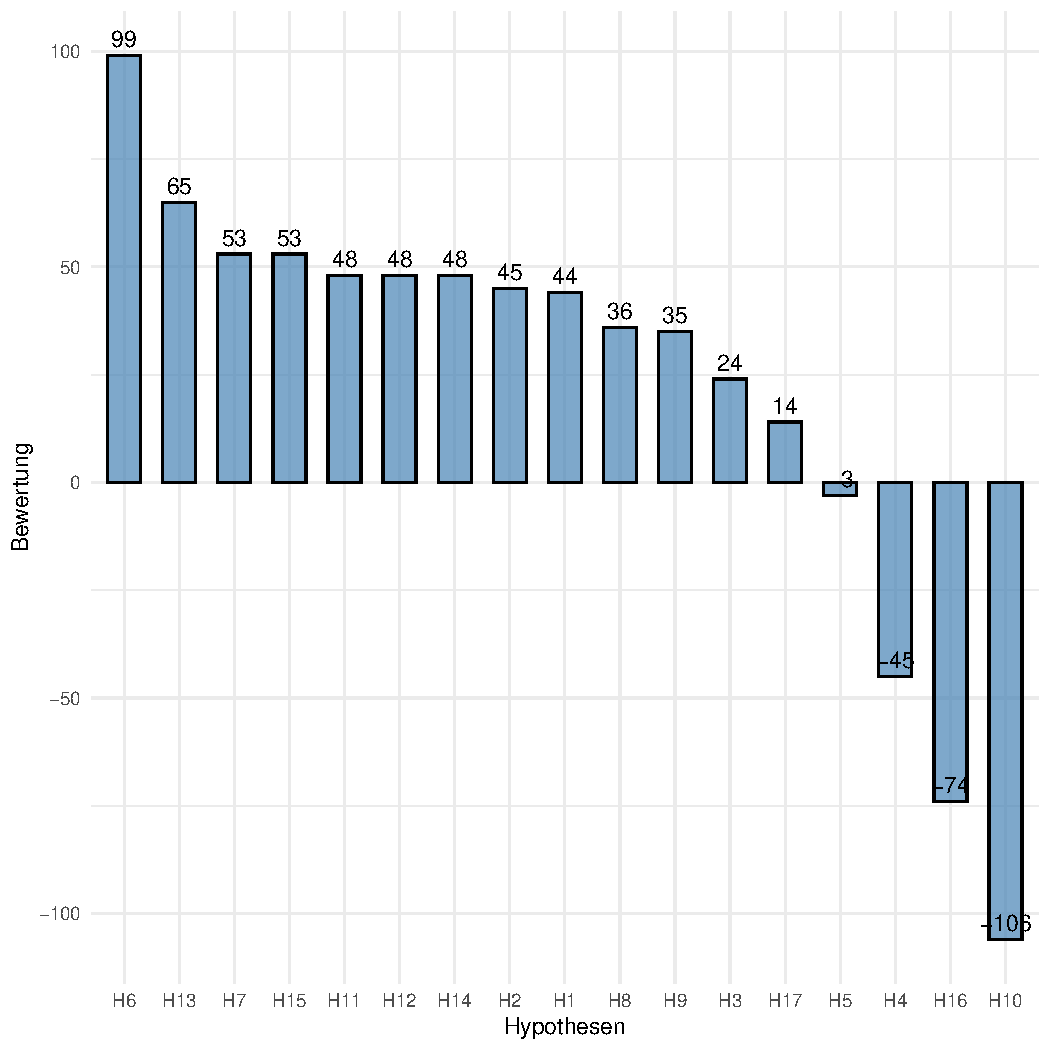
\includegraphics[width=0.8\columnwidth]{figures/plots/ranking.pdf}
\caption{\label{fig:ranking} Einstufung der Hypothesen nach Priorität}
\end{figure}

Nachdem die vorliegenden Daten analysiert sind, werden diese in einem letzten Schritt nach Wichtigkeit sortiert. Für dieses Verfahren ist die lineare Skala von 1 bis 5 auf $-2$ bis 2 abgebildet und ist pro Hypothese aufsummiert. Dies hat den Vorteil, dass Features, welche nicht benötigt werden, auch deutlich in der \autoref{fig:ranking} erkennbar sind. Die jeweilige Auswertung kann als Priorisierung für die einzelnen Aufgaben gesehen werden.

